\documentclass[12pt,a4paper]{article}

\usepackage[czech]{babel}
\usepackage{csquotes}
\usepackage{graphicx}
%\usepackage{textcomp}

% neodsazovat nové odstavce
\setlength{\parindent}{0pt}


\begin{document}

%%%%%%%%%%%%%%%% TITLE PAGE %%%%%%%%%%%%%%%%
\begin{titlepage}
	\begin{center}
		
\includegraphics[width=0.5\linewidth]{img/logo.pdf}
		\vspace{3cm}
			
		\LARGE\uppercase{Dokumentace 2. projektu IPK}
		\vspace{1cm}
			
		\LARGE\textbf{varianta ZETA: Sniffer Paketů}
			
		\vspace*{\fill}
		\large{Ondřej Mach (xmacho12)}
	\end{center}
\end{titlepage}
	
	
%%%%%%%%%%%%%%%% TABLE OF CONTENTS %%%%%%%%%%%%%%%%
\pagenumbering{arabic}
\setcounter{page}{1}
\tableofcontents
\clearpage
	
	
%%%%%%%%%%%%%%%% THE ACTUAL DOCUMENT %%%%%%%%%%%%%%%%

\section{Úvod}
Tento projekt se zabývá problematikou zachytávání paketů v počítačové síti.
Cílem tohoto projektu je implementace programu, který dokáže zachychovat pakety na vybraném rozhraní.
Tento program dále filtruje pakety podle protokolu a vypisuje čitelný výstup.
\newpage

\section{Implementace}
\subsection{Obecné údaje}
Program byl implementován v jazyce C++ s využitím knihovny \texttt{libpcap}.
Tato knihovna poskytuje high-level rozhraní zachycování paketů. Její implementace zpřístupní i pakety, které nejsou určeny pro daný počítač.
Libpcap je kompatibilní se systémy UNIXového typu i s Windows, tento projekt je však implementován s ohledem pouze na UNIX.
Vývoj probíhal na Linuxu, překlad byl otestován i na FreeBSD.

\subsection{Chování programu}
Program je spouštěn z příkazové řádky a svůj výstup posílá na \texttt{stdin}.
V případě jakékoli chyby (typicky nedostatečná oprávnění) vypíše chybovou hlášku na \texttt{stderr} a ukončí se.Každý zachycený paket se vypíše jako zpracované hlavičky a poté RAW data s přepisem do ASCII po straně.


Na linkové vrstvě (L2) program podporuje pouze Ethernet hlavičky.
Z nich jsou na výstup vypsány MAC adresy zdroje a cíle.


Na síťové vrstvě (L3) je již rozlišováno mezi IPv4, IPv6, ARP a ostatními pakety.
V případě, že je nalezena IPv4 nebo IPv6 hlavička, je na výstup vypsána IP adresa zdroje a cíle.

Na transportní vrstvě (L4) jsou podporovány protokoly TCP a UDP.
Pokud je jeden z nich rozpoznán, na výstup je zapsán zdrojový a cílový port.

\subsection{Struktura programu}
Celá struktura je přizpůsobena knihovně \texttt{libpcap}.
Po spuštění jsou nejprve parsovány argumenty pomocí funkce \texttt{getopt\_long} (GNU rozšíření \texttt{getopt}).

Dále se program pokusí otevřít dané síťové rozhraní, případně vypsat všechna dostupná rozhraní.

V další fázi běhu program zkompiluje zadaný filtr funkcí \texttt{pcap\_compile} a aplikuje ho na dané rozhraní.

Nakonec je spuštěna funkce \texttt{pcap\_loop}, která odchytí zadaný počet paketů a pro každý zavolá \texttt{packet\_callback}.
\texttt{packet\_callback} je nejdůležitější funkce v programu, která provádí samotnou analýzu paketů a jejich výpis.
Zde jsou používány i pomocné funkce, které vypisují data ve správných formátech.
Mezi ně patří třeba \texttt{formatTimestamp}, \texttt{formatMAC} nebo \texttt{formatIPv6}.
\newpage

\section{Testování}
\subsection{Nastavení}
Pro test v praxi byl vybrán protokol Telnet.
Dříve byl velmi hojně používaný pro vzdálenou správu, dokud nebyl nahrazen SSH.
Telnet je také nechvalně proslulý svým nešifrovaným provozem, proto je ideálním kandidátem k zachytávání paketů.
Test byl uskutečněn mezi hostitelským operačním systémem a hostem běžícím ve virtuálním stroji.
Na hostovi byl nainstalován a spuštěn telnet server.
Na hostiteli byl spuštěn wireshark a ipk-sniffer pro sledování provozu.
Nakonec se hostitel připojil přes telnet k serveru běžícímu na hostovi.

\subsection{Spuštění}
\begin{verbatim}
sudo ./ipk-sniffer -i virbr0 -n 100 -p 23
\end{verbatim}

ipk-sniffer je potřeba spouštět jako root, protože běžný uživatel nemá dostatečná oprávnění pro zachycování paketů.
Argument \texttt{-i} značí rozhraní, \texttt{-n} značí počet paketů.
Argument \texttt{-p} značí port - v tomto případě je použit port 23, což je standardní port pro Telnet.

Po zahájení spojení se na wiresharku i v našem snifferu začaly okamžitě ukazovat pakety.
Bohužel telnet není snadno čitelný a srozumitelný v ascii a uživatelský vstup chodí po jednom písmenu.
Byl vybrán jeden paket, ve kterém telnet server vypisuje zprávu před přihlášením.
Níže je umístěn screenshot tohoto paketu v ipk-snifferu v porovnání s Wiresharkem.
\newpage

\begin{center}
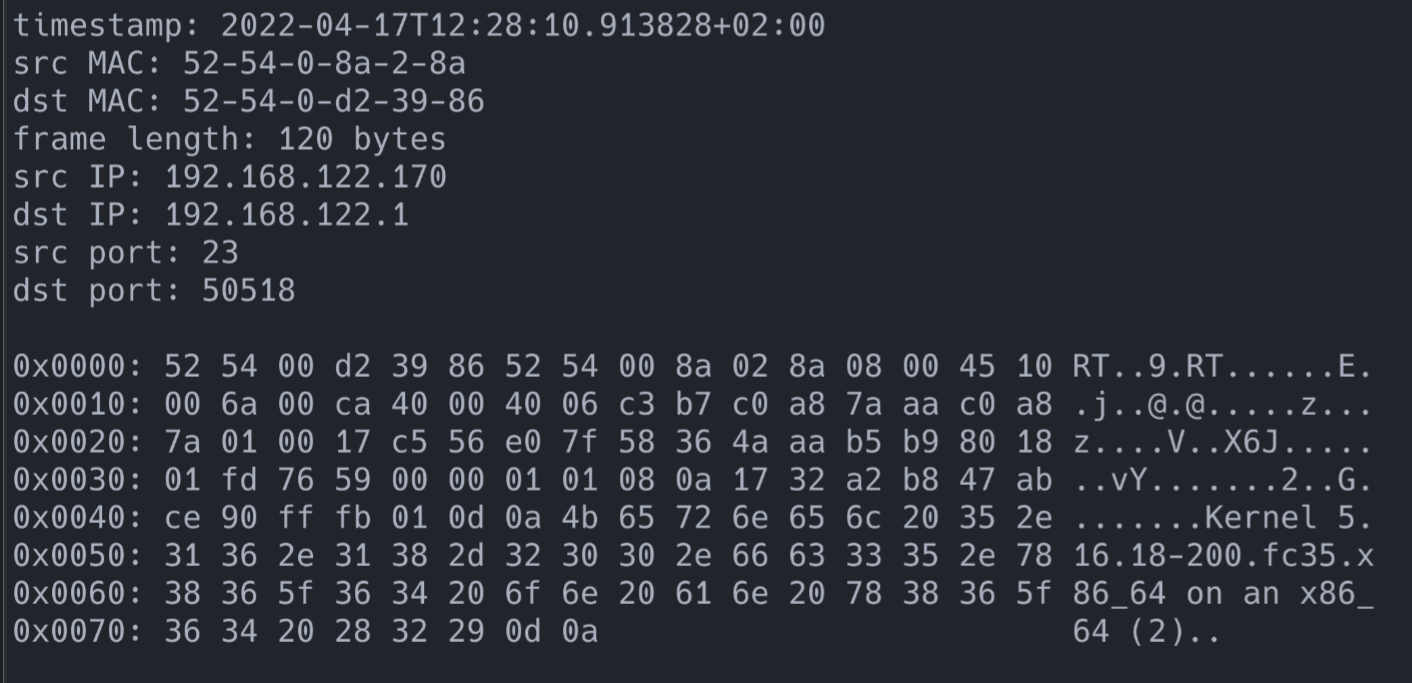
\includegraphics[width=0.7\linewidth]{img/welcome.png}  \\
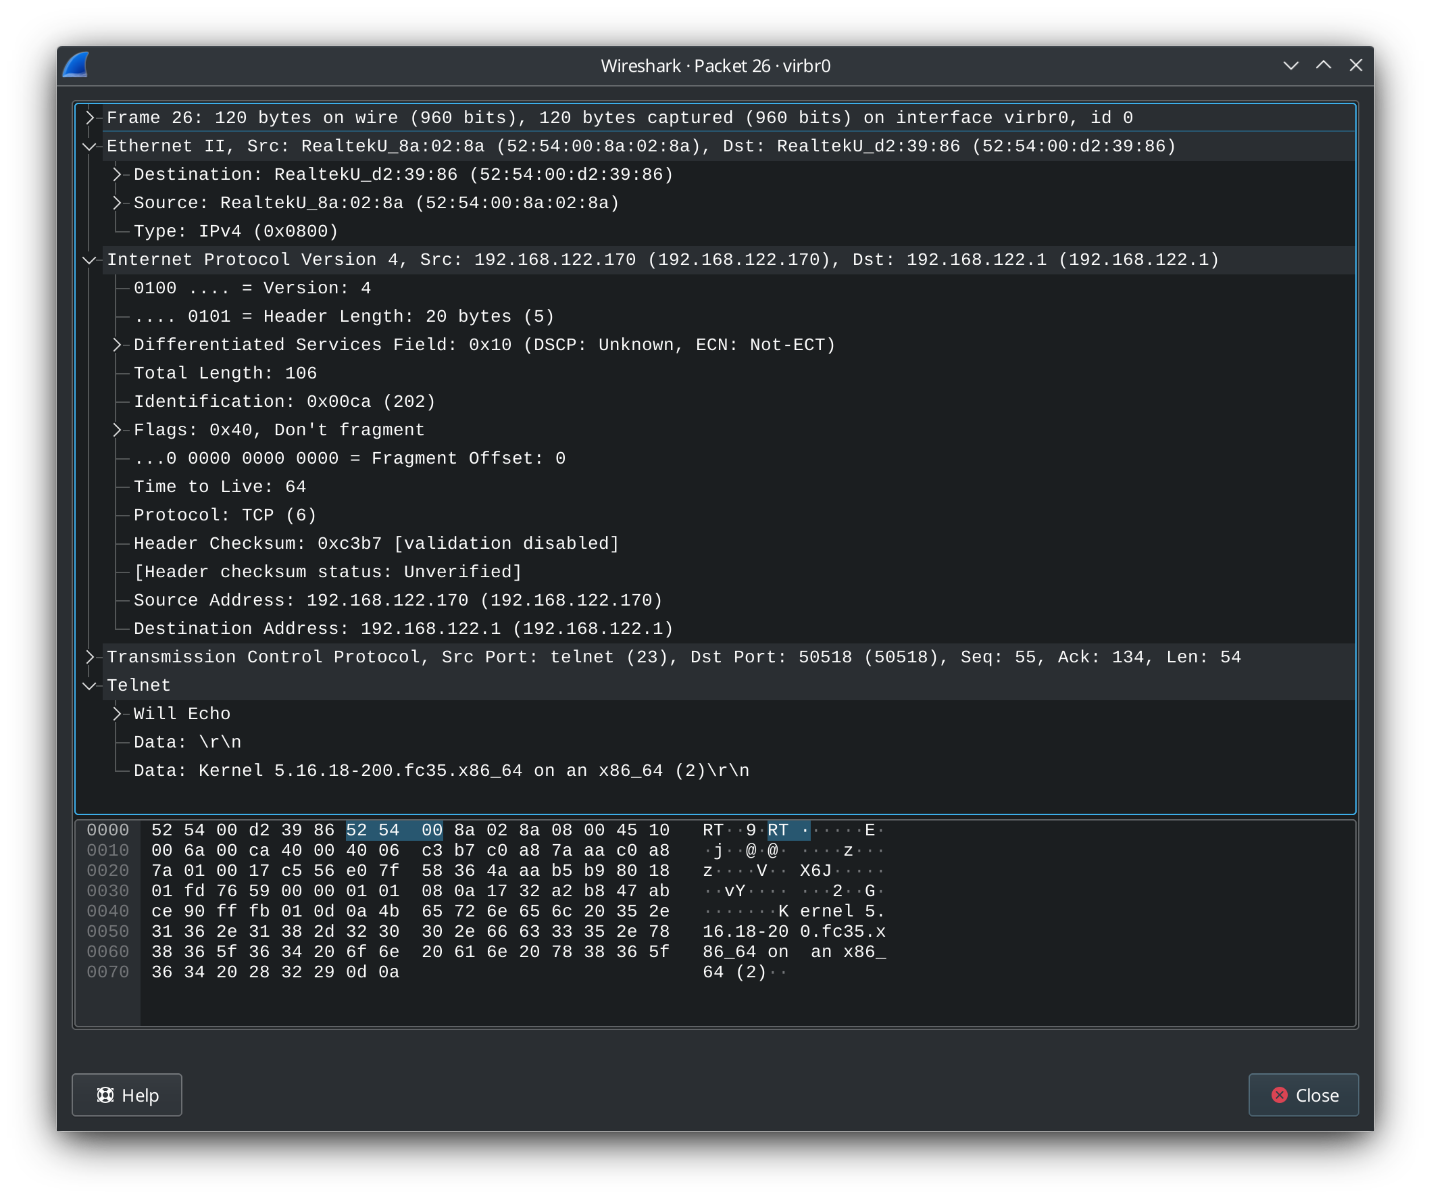
\includegraphics[width=1\linewidth]{img/welcome_wireshark.png}
\end{center}

Z výpisů je zřetelné, že se oba programy shodují na významu paketů a interpretaci headerů.
\newpage

Přestože v našem programu není příliš čitelné jaká data byla vyměněna, protokol není šifrovaný.
Proto je ve wiresharku funkce follow TCP stream, která sleduje data v paketech a poté je vypíše na jednu obrazovku (screenshot).

\begin{center}
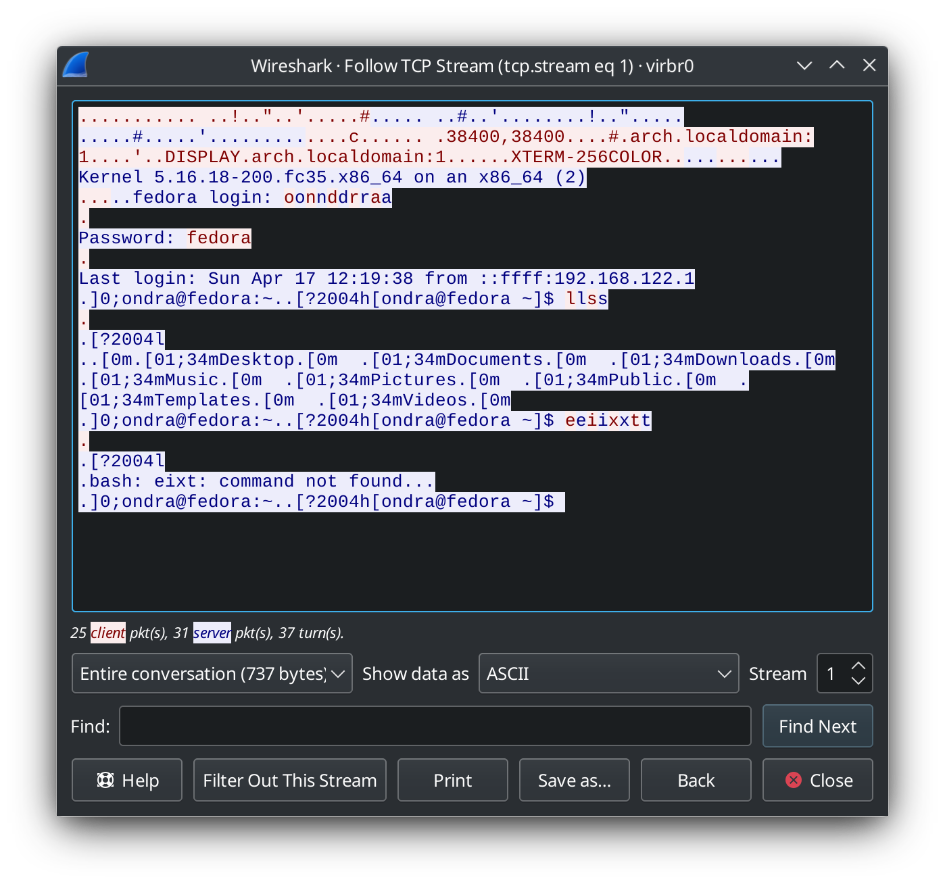
\includegraphics[width=1\linewidth]{img/follow.png}
\end{center}
\newpage



\end{document}
